\documentclass{article}

\usepackage[utf8]{inputenc}
\usepackage[brazilian]{babel}
\usepackage{graphicx}
\usepackage{float}
\usepackage[pdftex]{hyperref}
\usepackage{epstopdf}
\usepackage{etoolbox}
\usepackage{amsmath}
\usepackage{amsfonts}
\usepackage{amssymb}
\usepackage{caption}
\usepackage{subcaption}
\usepackage{setspace}
\usepackage{tikz}
\usepackage{listings}
\usepackage{xcolor} 

\patchcmd{\thebibliography}{\section*}{\section}{}{}
\newcommand{\R}{\ensuremath{\mathbb{R}}}
\newcommand{\Prob}{\ensuremath{\mathbb{P}}}
\newcommand{\K}{\ensuremath{\mathbb{K}}}
\newcommand{\U}{\ensuremath{\mathbb{U}}}
\newcommand{\N}{\ensuremath{\mathbb{N}}}
\newcommand{\Lg}{\ensuremath{\mathbb{L}}}
\newcommand{\T}{\ensuremath{\rm Tr}}
\newcommand{\sg}{{\sigma(x_k)}}

\newcommand{\G}{\ensuremath{\mathcal{G}}}
\newcommand{\F}{\ensuremath{\mathcal{F}}}
\newcommand{\C}{\ensuremath{\mathcal{C}}}
\newcommand{\E}{\ensuremath{\mathcal{E}}}
\newcommand{\Hn}{\ensuremath{\mathcal{H}}}
%\newcommand{\Hoo}{\ensuremath{\mathcal{H}_\infty}}
\newcommand{\Hop}{\ensuremath{\mathcal{H}_{op}}}
% --------------------------------------------------
\newtheorem{theo}{Teorema}
\newtheorem{exa}{Exemplo}
\newtheorem{lemm}{Lema}
\newtheorem{coro}{Corolário}
\newtheorem{defn}{Definição}[section]


%opening
\lstset{ %
	backgroundcolor=\color{black},   % choose the background color; you must add \usepackage{color} or \usepackage{xcolor}
	basicstyle=\footnotesize,        % the size of the fonts that are used for the code
	breakatwhitespace=false,         % sets if automatic breaks should only happen at whitespace
	breaklines=true,                 % sets automatic line breaking
	captionpos=t,                    % sets the caption-position to bottom
	commentstyle=\color{green},    % comment style
	extendedchars=true,              % lets you use non-ASCII characters; for 8-bits encodings only, does not work with UTF-8
	frame=single,                    % adds a frame around the code
	keepspaces=true,                 % keeps spaces in text, useful for keeping indentation of code (possibly needs columns=flexible)
	keywordstyle=\color{cyan},       % keyword style
	language=C,                 % the language of the code
	numbers=left,                    % where to put the line-numbers; possible values are (none, left, right)
	numbersep=5pt,                   % how far the line-numbers are from the code
	numberstyle=\tiny\color{black}, % the style that is used for the line-numbers
	rulecolor=\color{gray},         % if not set, the frame-color may be changed on line-breaks within not-black text (e.g. comments (green here))
	showspaces=false,                % show spaces everywhere adding particular underscores; it overrides 'showstringspaces'
	showstringspaces=false,          % underline spaces within strings only
	showtabs=false,                  % show tabs within strings adding particular underscores
	stepnumber=2,                    % the step between two line-numbers. If it's 1, each line will be numbered
	stringstyle=\color{red},     % string literal style
	tabsize=4,                       % sets default tabsize to 2 spaces
	basicstyle=\color{orange}
}

\begin{document}

\begin{titlepage}
\begin{center}

\newcommand{\HRule}{\rule{\linewidth}{0.5mm}}
% Upper part of the page. The '~' is needed because \\
% only works if a paragraph has started.

\includegraphics[width=0.15\textwidth]{logoUnicamp}~\\[1cm]

\textsc{\LARGE Universidade Estadual de Campinas}\\[1.5cm]

\textsc{\Large Faculdade de Engenharia Mecânica}\\[0.5cm]

% Title
\HRule \\[0.4cm]
{ \huge \bfseries ES670 - Projeto de Sistemas Embarcados\\ \vspace{1cm} Relatório - Projeto Prático (Parte 1/7) \\
\Large{Requisitos de Teclado, LEDs e Display de Sete Segmentos} \\[0.4cm] }

\HRule \\[1.5cm]

% Author and supervisor
\begin{minipage}{0.6\textwidth}
\begin{flushleft} \large
\emph{Nome:}\\
Rodolfo Nobre Bitu de Morais\\Guilherme de Oliveira Souza\\ Marcelli Tiemi Kian
\end{flushleft}
\end{minipage}
\begin{minipage}{0.2\textwidth}
\begin{flushright} \large
\emph{RA}\\ 105654\\117093\\
117892
\end{flushright}
\end{minipage}

\vfill

% Bottom of the page
{\large \today}

\end{center}
\end{titlepage}


\onehalfspacing
\section{Objetivo} 
O objetivo do projeto é, de maneira incremental, implementar no target os requisitos apresentados no roteiro\cite{bb:roteiro} inicialmente desenvolvendo o modelo e depois implementando cada requisito. Estes requisitos são referentes à configuração e implementação de entradas de teclado, acionamento de LEDs, display de sete segmentos, protocolo de comunicação, display LCD, medição de velocidade de rotação, PWM, ADC e Controlador. 
	
\section{Modelagem}
% Diagramas requisitos implementados, digrama de blocos, etc
Utilizando o Rational Rhapsody Modeler e tomando como base os requisitos propostos mostrados na figura \ref{fig:requisitos}, complementamos o modelo inicial\cite{bb:modelo} (requisitos de teclado e LEDs) adicionando um bloco ao modelo referente aos displays de sete segmentos (REQ1C), conforme mostrado na figura \ref{fig:blocos}.

\begin{figure}[H]
	\centering
	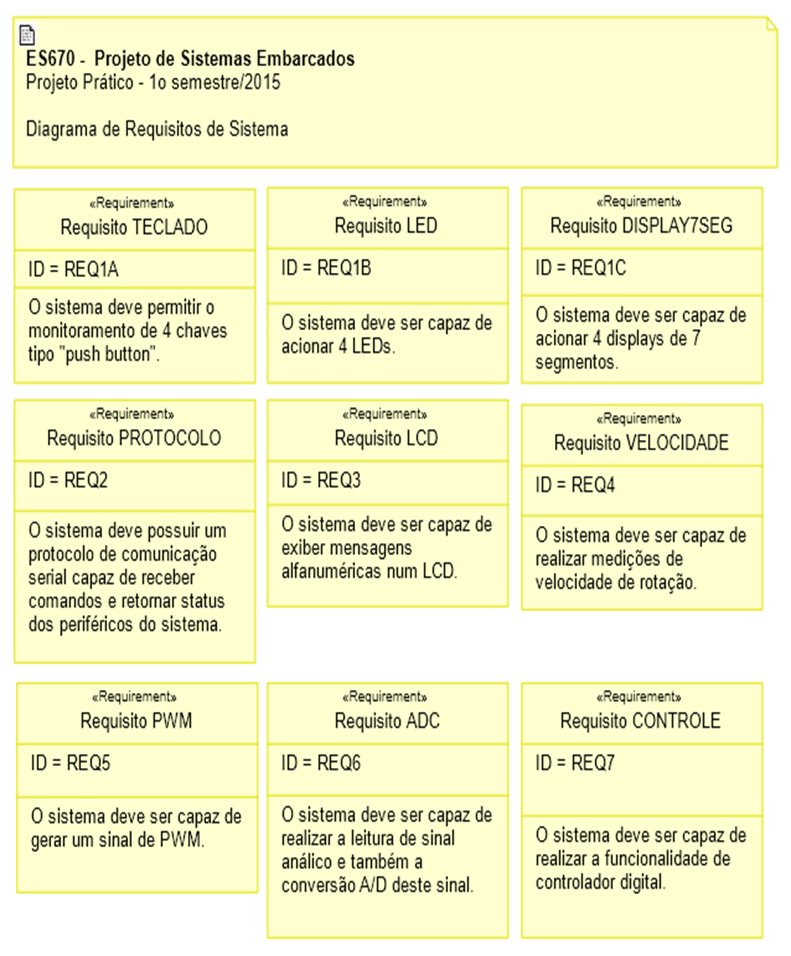
\includegraphics[width=0.9\linewidth]{requisitos}
	\caption{Diagrama de requisitos}
	\label{fig:requisitos}
\end{figure}
\begin{figure}[H]
	\centering
	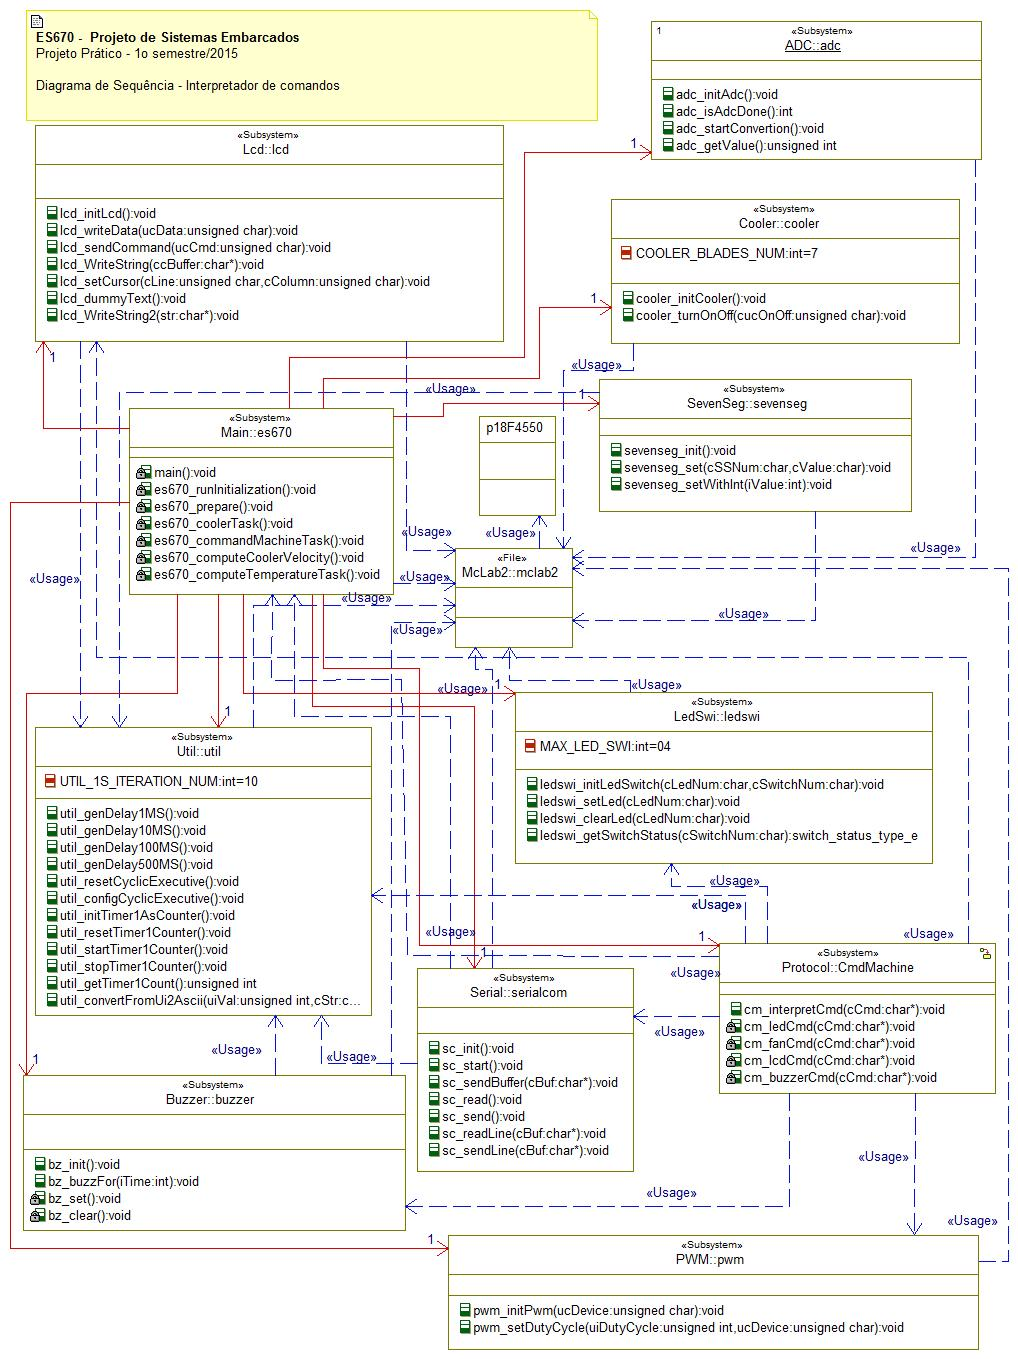
\includegraphics[width=0.9\linewidth]{blocos}
	\caption{Diagrama de definição de blocos}
	\label{fig:blocos}
\end{figure}
O bloco ``SevenSeg'' possui três operações: inicialização, definição de saída (recebendo qual dos displays será usado e qual valor deve ser exibido) e definição de saída com inteiro (recebendo apenas o valor inteiro a ser exibido no conjunto de quatro displays).

Com o objetivo de cumprir o requisito de comunicação serial (REQ2), foram adicionados os blocos Serial e CmdMachine. O bloco ``Serial'' é o bloco responsável pela comunicação serial simples, tendo como funções mandar e receber as mensagens. O bloco ``CmdMachine'' já tem a função de interpretar o que é recebido pela porta serial. Ainda foi adicionado o bloco ``Buzzer'', que controla o funcionamento do buzzer do kit.

Para cumprir o requisito de exibir mensagens no display LCD, foi adicionado o bloco ``LCD'', responsável pela configuração inicial do hardware do dispositivo e implementação de uma interface de mais alto nível para mandar mensagens no formato de string para o componente.

O requisito para medição de velocidade de rotação (REQ4) foi cumprido com o bloco ``Cooler'' e no próprio bloco ``ES670\_pp''. O bloco ``cooler'' configura o hardware para a utilização do cooler e controla o estado ligado e desligado.

O requisito para acionar o cooler com PWM (REQ5) foi cumprido com o bloco ``pwm'', responsável por fazer a configuração inicial do dispositivo e tambem por ajustar o duty cycle durante a execução.

Ainda foi adicionado no ``ES670\_pp''o executivo cíclico cooperativo, então foram colocadas 6 tasks:
\begin{description}
\item[Compute Cooler Velocity] calcula a velocidade do cooler, utilizando sensores infravermelho
\item[Cooler] controla o estado do cooler
\item[Command Machine] interpreta os comandos enviados por serial
\item[Compute Temperature] calcula a temperatura
\item[Display] atualiza o display LCD
\item[Control] implementa um controlador PID
\end{description}

O requisito de fazer leitura de um sinal analógico e fazer conversão A/D do sinal (REQ6) foi cumprido usando um aquecedor e um sensor de temperatura. O blcoo ``adc'' lê o sinal analógico e faz sua conversão utilizando uma máquina de estados, pois o ADC precisa de um certo tempo para terminar de fazer a conversão.

A informação da converesão então é salva e é mostrada no LCD quando solicitado pelo usuário via comunicação serial.

\section{Diagramas Esquemáticos}
% Diagramas esquemáticos do target utilizados

\begin{figure}[H]
	\centering
	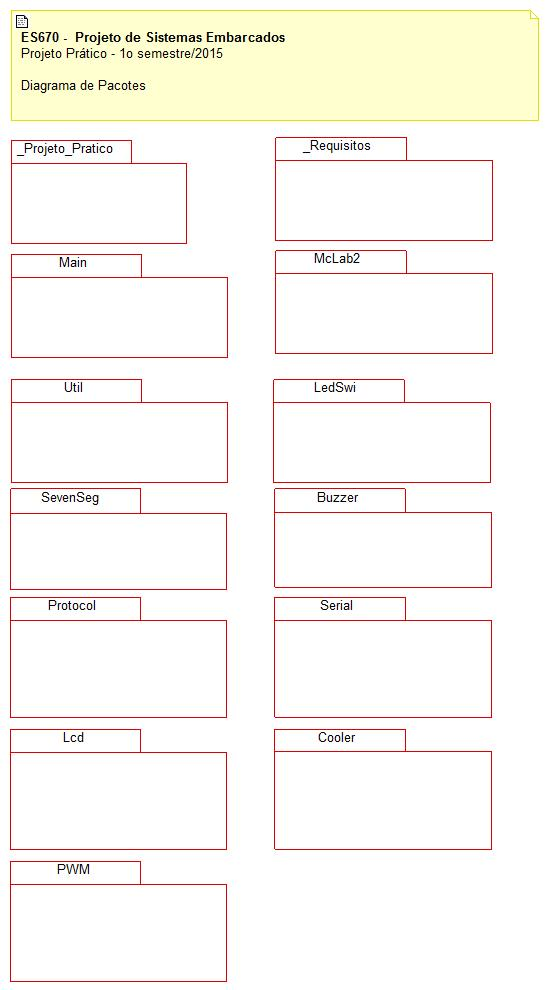
\includegraphics[width=0.7\linewidth]{pacotes}
	\caption{Diagrama de pacotes}
	\label{fig:pacotes}
\end{figure}
\begin{figure}[H]
	\centering
	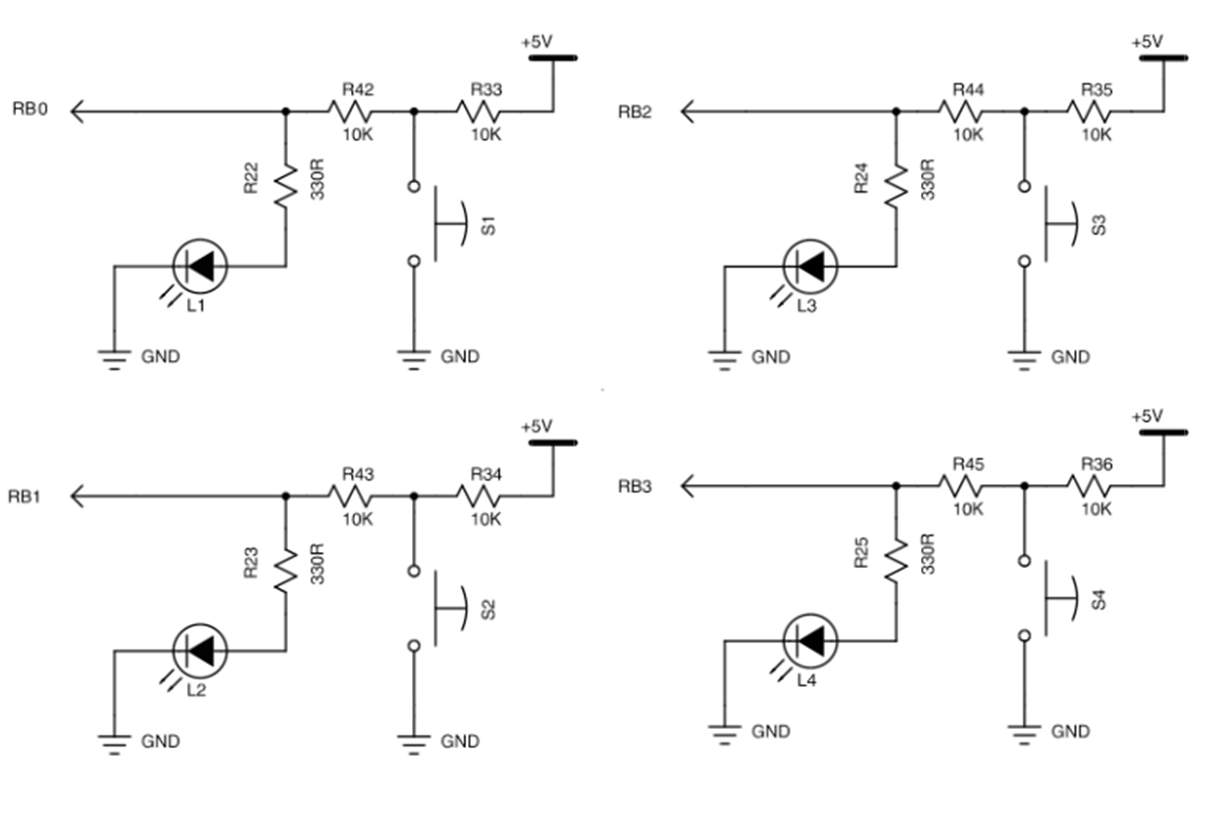
\includegraphics[width=0.7\linewidth]{esq_ledswi}
	\caption{Esquema teclado e LEDs}
	\label{fig:esq_ledswi}
\end{figure}
\begin{figure}[H]
	\centering
	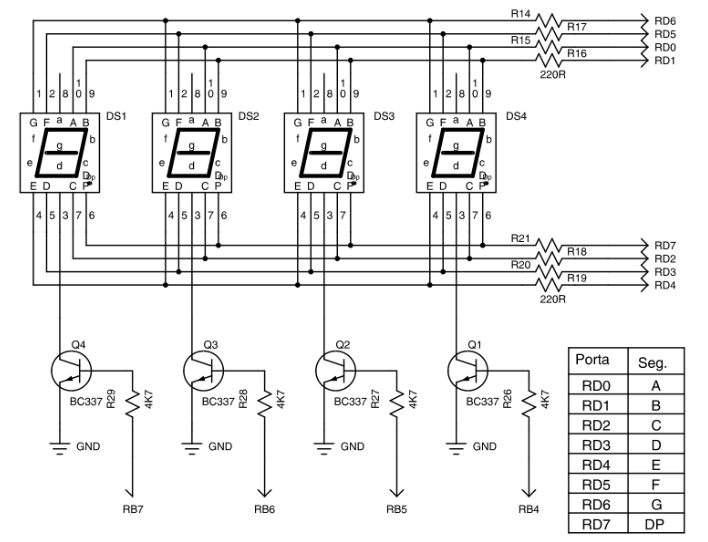
\includegraphics[width=0.9\linewidth]{esq_7seg}
	\caption{Esquema sete segmentos}
	\label{fig:esq_7seg}
\end{figure}
\begin{figure}[H]
	\centering
	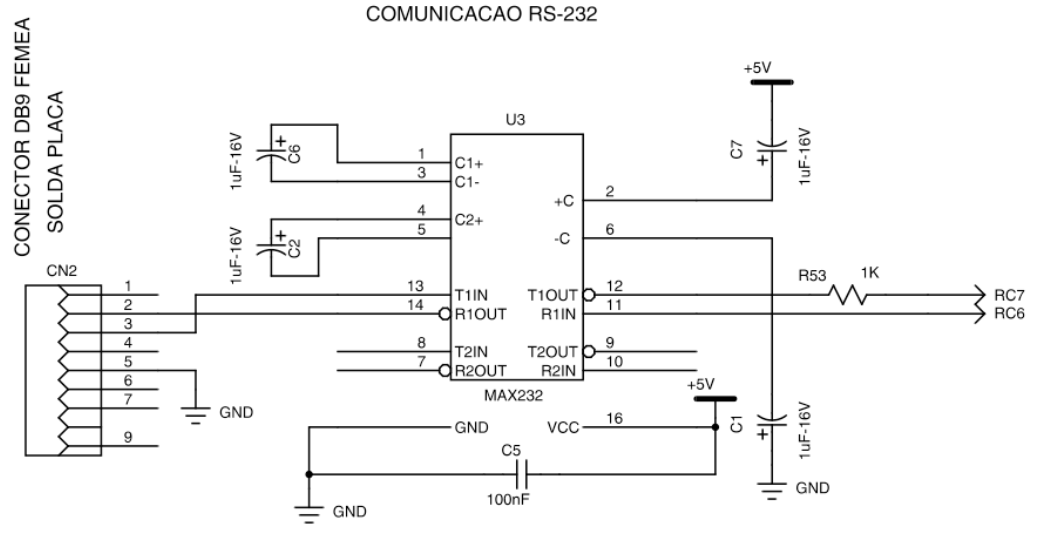
\includegraphics[width=0.9\linewidth]{serial}
	\caption{Esquema comunicação serial}
	\label{fig:serial}
\end{figure}
\begin{figure}[H]
	\centering
	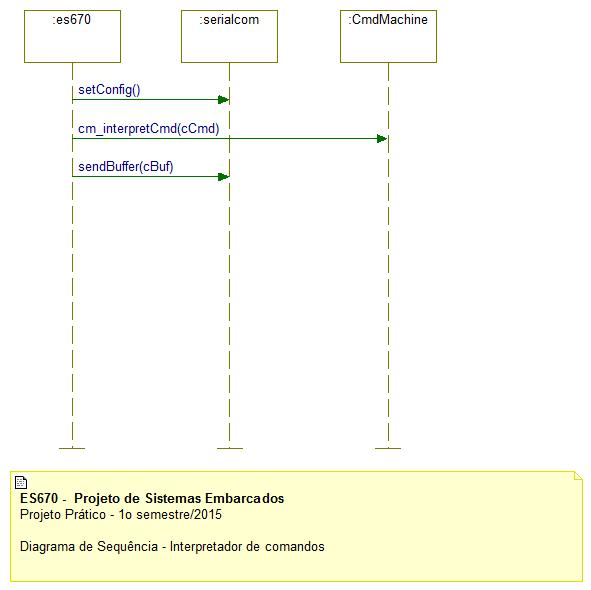
\includegraphics[width=0.9\linewidth]{interpretador}
	\caption{Esquema do interpretador de comandos}
	\label{fig:interpretador}
\end{figure}
\begin{figure}[H]
	\centering
	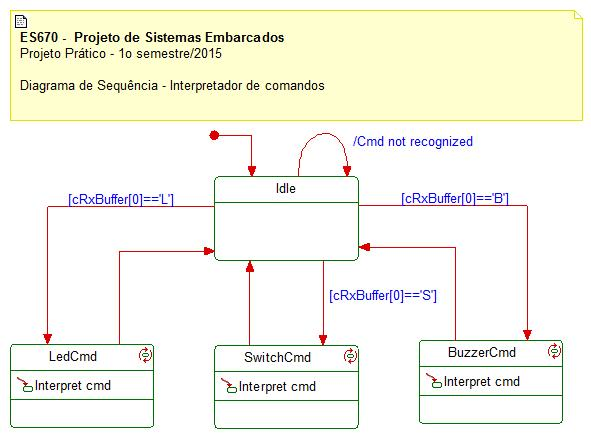
\includegraphics[width=0.9\linewidth]{maquina}
	\caption{Esquema da máquina de estados para interpretação de comandos}
	\label{fig:maquina}
\end{figure}
\begin{figure}[H]
	\centering
	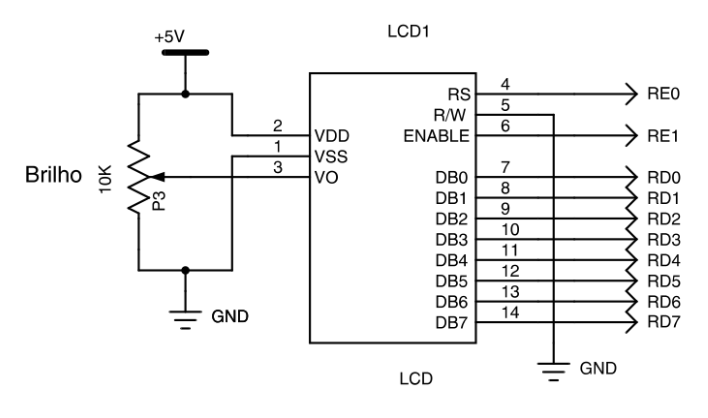
\includegraphics[width=0.9\linewidth]{esq_lcd}
	\caption{Esquema do componente LCD}
	\label{fig:esq_lcd}
\end{figure}
\begin{figure}[H]
	\centering
	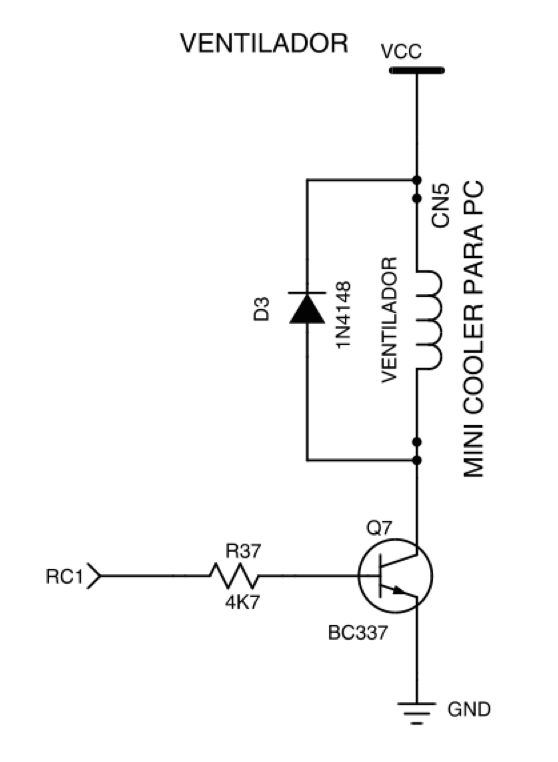
\includegraphics[width=0.5\linewidth]{esq_cooler}
	\caption{Esquema do ventilador}
	\label{fig:esq_cooler}
\end{figure}
\begin{figure}[H]
	\centering
	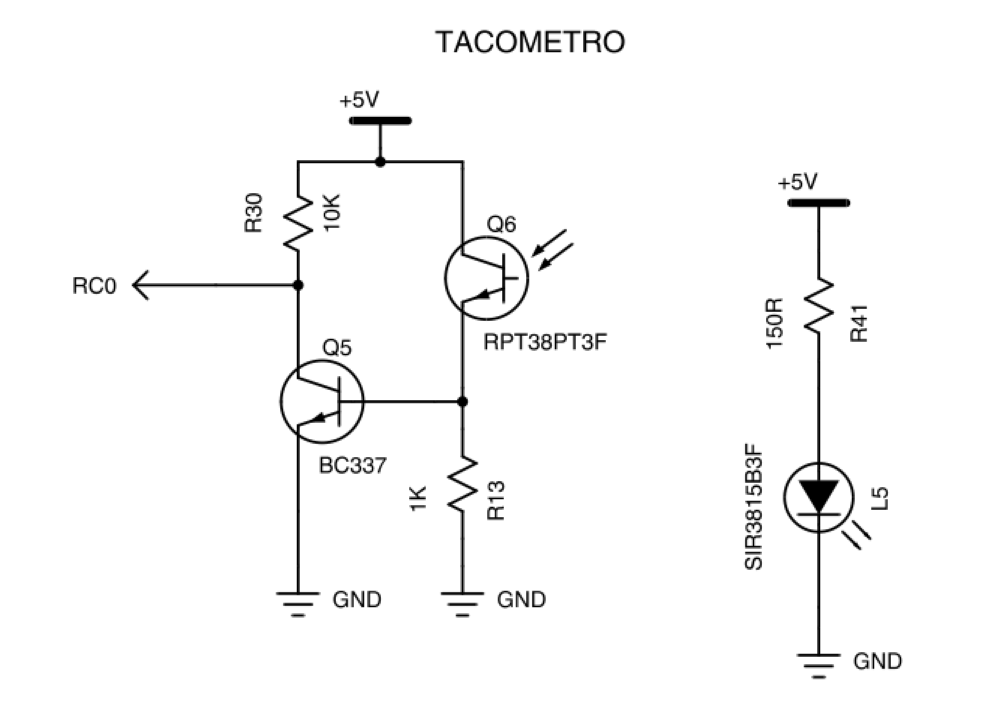
\includegraphics[width=0.9\linewidth]{esq_sensor}
	\caption{Esquema do tacômetro}
	\label{fig:esq_sensor}
\end{figure}
\begin{figure}[H]
	\centering
	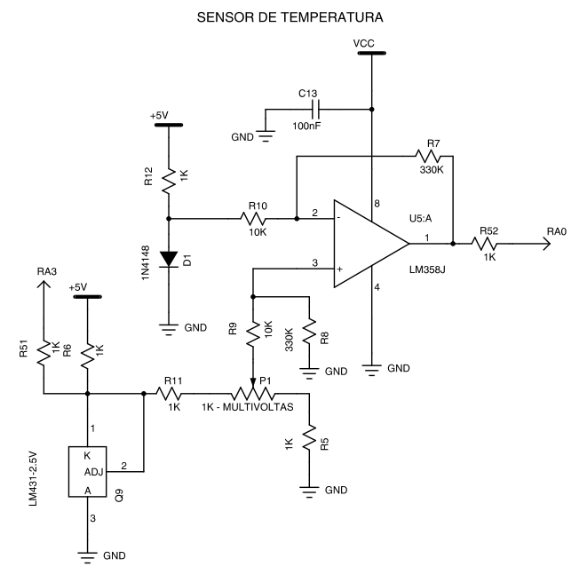
\includegraphics[width=0.9\linewidth]{esq_sensorTemp}
	\caption{Esquema do sensor de temperatura}
	\label{fig:esq_sesorTemp}
\end{figure}
\begin{figure}[H]
	\centering
	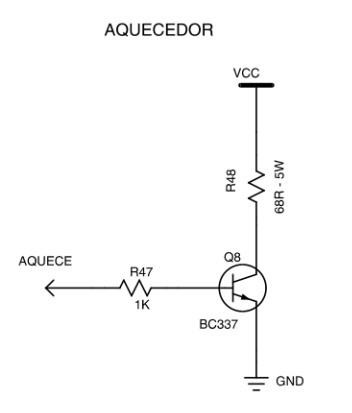
\includegraphics[width=0.9\linewidth]{esq_aquecedor}
	\caption{Esquema do aquecedor}
	\label{fig:esq_aquecedor}
\end{figure}

Como pode ser visto na figura \ref{fig:esq_7seg}, é necessário fazer um gerenciamento das portas RB4-7 e RD0-7 para que sejam mostrados os valores desejados nos displays de sete segmentos. Para isso, é preciso alternar qual RB está ativo fazendo a mudança nos RD0-7 para que cada display esteja mostrando um valor diferente. É importante lembrar que a frequência dessa alternância seja escolhida de modo que o olho humano não perceba que os displays estão ligando e desligando.

Observando a figura \ref{fig:serial}, para a manipulação da comunicação serial é necessário fazer a configuração inicial das portas TXSTA, RCSTA e BAUDCON e dos bits RC7 e RC6 para que a comunicação serial funcione da forma apropriada para nossa utilização.  Para enviar através da porta serial, é necessário que o bit TXIF da porta PIR1 esteja TRUE e colocar o que será enviado em TXREG. Para receber, é necessário que o bit RCIF da porta PIR1 esteja TRUE e ler RCREG.

\section{Implementação da sintaxe do protocolo de comunicação}

Após a leitura dos dados recebidos pela função ``sc\_receiveBuffer'', o comando é interpretado pela função ``cm\_interpretCmd'' e então é executado um determinado comportamento. Como é possível ver na figura \ref{fig:maquina}, o interpretador lê a primeira letra e trata o restante das informações recebidas de maneira diferente.

A sintaxe para comunicação é definida como:
\begin{itemize}
\item L[CS][1-4] - Comanda um led [1-4] para ligar ou desligar [CS], onde C é clear e S é set.
\item S[1-4] - Retorna o estado do switch [1-4]. A resposta é dada como aberta ou fechada [OC], onde O é opened e C é closed.
\item Bx - Onde x é um inteiro, comanda o buzzer para ligar durante x milissegundos.
\item LCDccccc - Onde ccccc é uma sequência de no máximo 32 caracteres que deve ser exibida no LCD
\item SPD - Mostra no LCD a velocidade do ventilador (cooler) em tempo real e a temperatura do aquecedor
\item FANddd - Ajusta o duty cycle para o valor (entre 0 e 100) desejado
\item HTRddd - Ajusta o duty cycle do resistor
\item REFdd - Ajusta a temperatura de referência usada no controle
\end{itemize}

Apesar de estar no modelo, a implementação do Switch ainda não está completa.

\section{Executivo cíclico cooperativo}

Para fazer o executivo cíclico cooperativo, foram implementadas tasks para executar as tarefas que cumprem os requisitos.

\subsection{Período do PWM}
No arquivo pwm, o período do PWM é ajustado para 46.875 kHz. Para obter esse valor, o registrador PR2 é escrito com o valor da fórmula abaixo

\begin{equation}
PR2 = \frac{Period}{4*Tosc*pre}-1 = 255
\end{equation}

\subsection{Cálculo da velocidade}
No arquivo es670\_pp é chamado ``es670\_computeCoolerVelocity", sua função é atualizar o valor da velocidade do cooler. Um vetor cíclico de 10 posições é usado para guardar o histórico e esse mesmo valor é usado para calcular a velocidade. Ainda é avisado para a Máquina de Estados o valor atual da velocidade.

\subsection{Controle do estado do ventilador}
No arquivo es670\_pp é chamado de ``es670\_coolerTask'', sua função é desligar ou ligar o cooler a partir da entrada que é fornecida a partir do botão apertado.
Futuramente, queremos remover essa task e adicioná-la à Máquina de Estados.

\subsection{Chamada para a Máquina de Estados}
No arquivo es670\_pp é chamado de ``es670\_commandMachineTask'', sua função é acionar a máquina de estados a partir de um buffer que é preenchido quando a interrupção é chamada a partir do serial. Ela ainda verifica se deve ou não continuar mostrando e atualizando a velocidade do cooler e a temperatura no LCD.

\subsection{Cálculo da temperatura}
No arquivo es670\_pp é chamado ``es670\_computeTemperatureTask'', sua função é gerenciar o conversor analógico-digital para o cálculo da temperatura.
A task é logicamente dividida em três etapas, todas executadas no mesmo ciclo:
\begin{itemize}
\item Inicio: Onde é feito o começo da conversão do ADC;
\item Convertendo: Onde é feita a espera pelo resultado da conversão ADC;
\item Fim: Onde é usado o valor retornado pelo ADC para fazer o cálculo da temperatura em ºC.
\end{itemize}

\subsection{As interrupções}
O tratamento de interrupções pode ser visto no arquivo es670\_pp em ``isr\_CyclicExecutive''. As interrupções tratadas estão listadas abaixo:
\begin{itemize}
\item Timer1: A interrupção do timer1, utilizada para fazer o cálculo da velocidade do cooler, pois o o timer1 é como contador.
\item Leitura serial: Essa interrupção é utilizada para que o buffer utilizado pela Máquina de Estados seja preenchido com o que é recebido pelo serial. Sempre que um caractere novo é recebido, o buffer deve ser atualizado.
\item Envio serial: Essa interrupção é utilizada para enviar informações através da porta serial sem comprometer o executivo cíclico cooperativo. Sempre que um caractere novo pode ser enviado, ele é enviado.
\end{itemize}

\subsection{Controle de temperatura}
O controle da temperatura do resistor é feito acionando o cooler da placa e coletando a temperatura através do diodo.

A cada ciclo, o valor atual da leitura da temperatura é usado para obter o esforço de controle necessário.

O controlador utilizado é um controlador PID, com ganhos $K_p$, $K_i$ e $K_d$ definidos em tempo de compilação, calibrados manualmente. Os valores usados para nosso target foi:

\begin{align*}
K_p &= 50\\
K_i &= 0.5\\
K_d &= 0
\end{align*}

O esforço de controle é obtido pela seguinte fórmula:

\begin{equation}
C = - (K_p * ErroInstantaneo + K_i * ErroAcumulado + K_d * Variacao)
\end{equation}

O sinal negativo na fórmula se dá ao fato de que o atuador (cooler) se opõe à variável controlada (temperatura).

\section{Matriz de Rastreabilidade}
% Matriz de rastreabilidade de requisitos vs implementações
A matriz de rastreabilidade apresentada na tabela \ref*{tab:rastreabilidade} relaciona cada um dos requisitos com a sua implementação.
\begin{table}[H]
	\centering
	\caption{Matriz de Rastreabilidade}
	\label{tab:rastreabilidade}
	\small
	\begin{tabular}{|c|l|}
		\hline \bfseries{ID do Requisito} & \bfseries{Implementação}\\ 
		\hline REQ1A 	& \texttt{ledswi.c}\\ 
						& \texttt{- void ledswi\_initLedSwitch(char cLedNum, char cSwitchNum)}\\
						& \texttt{- switch\_status\_type\_e ledswi\_getSwitchStatus(char cSwitchNum)}\\
		\hline REQ1B 	& \texttt{ledswi.c}\\ 
						& \texttt{- void ledswi\_initLedSwitch(char cLedNum, char cSwitchNum)}\\
						& \texttt{- void ledswi\_setLed(char cLedNum)}\\ 
						& \texttt{- void ledswi\_clearLed(char cLedNum)}\\
		\hline REQ1C 	& \texttt{sevenSeg.c}\\ 
						& \texttt{- void sevenseg\_init(void)}\\
						& \texttt{- void sevenseg\_set(char cSSNum, sevenseg\_value\_e eValue)}\\
						& \texttt{- void sevenseg\_setWithInt (int iValue)}\\
		\hline REQ2	 	& \texttt{serialcom.c}\\ 
						& \texttt{- void sc\_init(void)}\\
						& \texttt{- void sc\_start(void)}\\
						& \texttt{- void sc\_sendBuffer(char cBuf[])}\\
						& \texttt{- void sc\_receiveBuffer(char cBuf[])}\\
						& \texttt{cmdMachine.c}\\ 
						& \texttt{- void cm\_interpretCmd(char cCmd[])}\\
		\hline REQ3	 	& \texttt{lcd.c}\\ 
						& \texttt{- void lcd\_initLcd(void)}\\
						& \texttt{- void lcd\_WriteString2(char str[])}\\
						& \texttt{- void lcd\_write2Lcd(unsigned char ucBuffer,  unsigned char cDataType)}\\
						& \texttt{- void lcd\_writeData(unsigned char ucData)}\\
						& \texttt{- void lcd\_sendCommand(unsigned char ucCmd)}\\
						& \texttt{- void lcd\_setCursor(unsigned char cLine, unsigned char cColumn)}\\
						& \texttt{cmdMachine.c}\\ 
						& \texttt{- void cm\_lcdCmd(char cCmd[])}\\
   	    \hline REQ4    	& \texttt{es670\_pp.c}\\
       	           		& \texttt{- void es670\_coolerTask(void)}\\
     					& \texttt{- void es670\_commandMachineTask(void)}\\
						& \texttt{- void es670\_computeCoolerVelocity(void)}\\
						& \texttt{- void isr\_CyclicExecutive(void)}\\
						& \texttt{cooler.c}\\
						& \texttt{- void cooler\_initCooler(void)}\\
						& \texttt{- void cooler\_turnOnOff(const unsigned char cucOnOff)}\\
       	\hline REQ5     & \texttt{pwm.c}\\
						& \texttt{- void pwm\_initPwm(void)}\\
						& \texttt{- void pwm\_setDutyCycle(const unsigned int uiDutyCycle)}\\
						& \texttt{cmdMachine.c}\\
						& \texttt{- void cm\_fanCmd(char cCmd[])}\\
       	\hline REQ6    	& \texttt{es670\_pp.c}\\
						& \texttt{- void es670\_computeTemperatureTask(void)}\\
						& \texttt{adc.c}\\
						& \texttt{- void adc\_initAdc(void)}\\
						& \texttt{- int adc\_isAdcDone(void)}\\
						& \texttt{- void adc\_startConvertion(void)}\\
						& \texttt{- unsigned int adc\_getValue(void)}\\
		\hline REQ7		& \texttt{es670\_pp.c}\\
						& \texttt{- void es670\_controlTask(void)}\\
						& \texttt{pid.c}\\
						& \texttt{ - PID pid\_init(double dP, double dI, double dD)}\\
						& \texttt{ - double pid\_update(PID *pid, double dRef, double dSensorValue)}\\
		\hline
	\end{tabular} 
	\normalsize
\end{table}
\section{Notas}
% Dificuldades, observações relevantes, correções, ...
Os maiores problemas identificados foram a dificuldade de conseguir conectar a placa com o computador e alguns mal contatos relacionados aos botões e do próprio PIC. Além disso, houve alguns conflitos com a IDE, pois muitas funcionalidades poderiam ter sido implementadas, já que a função de autocompletar é bem comum em IDE's e o duplo clique poderia selecionar a palavra em vez de colocar um breakpoint.

Tivemos problemas com relação ao tempo, pois tentamos implementar as três funções que foram pedidas inicialmente para a porta serial, mas só conseguimos colocar a função do LED para funcionar e a função do Buzzer estava quase pronta, mas não conseguimos a tempo. Colocamos no modelo, mas a implementação estava incompleta. Depois, com mais tempo, voltamos e implementamos essa funcionalidade.

Na implementação do comando de exibição no LCD tivemos problema por não esperar algum tempo após enviar o comando de limpar o display para enviar os dados a serem exibidos. Sem essa espera, parte do conteúdo era ``engolido''.

Durante a implementação do executivo cíclico cooperativo, reparamos que o restante da implementação anterior não encaixava na ideia do ciclo, portanto precisamos fazer adaptações nas implementações anteriores para fazer que os requisitos anteriores continuassem a ser cumpridos. Apesar de termos conseguido resultados positivos, ainda não resolvermos o problema do buzzer, pois ele ainda está tomando o processo para si enquanto está ativo. Pretendemos usar um timer e sua interrupção para resolver isso, mas ainda não vimos se ainda há um terceiro timer ou precisaremos criar alguma outra solução (timer2 está reservado para o PWM).

Durante os testes iniciais do cooler com acionamento usando PWM, ele pareceu não funcionar. Depois descobrimos que um leve empurrão era suficiente para desemperrá-lo e fazê-lo começar a girar.

\begin{thebibliography}{widestlabel}
	\bibitem{bb:roteiro}{Roteiro de Laboratório - Semanas 04 e 05 (disponibilizado para os alunos)}
	\bibitem{bb:modelo}{Projeto do Modelo Inicial do Sistema (disponibilizado para os alunos)}
	\bibitem{bb:codigo}{Código Fonte Inicial em Linguagem C (disponibilizado para os alunos)}
	\bibitem{bb:github}{Código Fonte no\href{https://github.com/rodolfobitu/Barco/tree/2333be0fed3d00b446ad03ea57678992bfadc12a}{GitHub}}

\end{thebibliography}

\section{Apêndice}
% Colocar como apêndice toda a listagem do código fonte
Listagem dos códigos fonte:
\lstinputlisting[language=C, title = \lstname]{../headers/ledswi.h}
\lstinputlisting[language=C, title = \lstname]{../src/ledswi.c}
\lstinputlisting[language=C, title = \lstname]{../headers/es670_pp.h}
\lstinputlisting[language=C, title = \lstname]{../src/es670_pp.c}
\lstinputlisting[language=C, title = \lstname]{../headers/mclab2.h}
\lstinputlisting[language=C, title = \lstname]{../headers/util.h}
\lstinputlisting[language=C, title = \lstname]{../src/util.c}
\lstinputlisting[language=C, title = \lstname]{../headers/sevenSeg.h}
\lstinputlisting[language=C, title = \lstname]{../src/sevenSeg.c}
\lstinputlisting[language=C, title = \lstname]{../headers/cmdMachine.h}
\lstinputlisting[language=C, title = \lstname]{../src/cmdMachine.c}
\lstinputlisting[language=C, title = \lstname]{../headers/serialcom.h}
\lstinputlisting[language=C, title = \lstname]{../src/serialcom.c}
\lstinputlisting[language=C, title = \lstname]{../headers/buzzer.h}
\lstinputlisting[language=C, title = \lstname]{../src/buzzer.c}
\lstinputlisting[language=C, title = \lstname]{../headers/lcd.h}
\lstinputlisting[language=C, title = \lstname]{../src/lcd.c}
\lstinputlisting[language=C, title = \lstname]{../headers/cooler.h}
\lstinputlisting[language=C, title = \lstname]{../src/cooler.c}
\lstinputlisting[language=C, title = \lstname]{../headers/pwm.h}
\lstinputlisting[language=C, title = \lstname]{../src/pwm.c}
\lstinputlisting[language=C, title = \lstname]{../headers/adc.h}
\lstinputlisting[language=C, title = \lstname]{../src/adc.c}
\lstinputlisting[language=C, title = \lstname]{../headers/pid.h}
\lstinputlisting[language=C, title = \lstname]{../src/pid.c}

\end{document}

